\section{Biases and uncertainties of the existing transformation models 现有转换模型的偏差和不确定性}

\begin{Parallel}{0.60\textwidth}{}
    \ParallelLText
    {
        The bias factors and coefficients of variation (COVs) of all models with respect to the global database are calibrated, except the three models that are only presented as graphical curves in the literature. The bias factor is denoted by $b$, and the COV is denoted by $\delta$. Basically, $b$ is the sample mean of (actual target value)/(predicted target value) for the global data points, and $\delta$ is the sample COV of (actual target value)/(predicted target value). For instance, for the $\rm{LI}-(s_u^{re}/P_a)$ model proposed by \citet{Locat1988799}, the actual target value is the $s_u^{re}/P_a$ value in the global database, and the predicted target value is $0.0144\rm{LI}^{-2.44}$. For each data point with simultaneous knowledge of $(\rm{LI},~s_u^{re})$, (actual target value)/(predicted target value) = $(s_u^{re}/P_a)/(0.0144\rm{LI}^{-2.44})$ can be computed. The histogram of the ratio $(s_u^{re}/P_a)/(0.0144\rm{LI}^{-2.44})$ is plotted in Fig. \ref{figure:15}. The sample mean of this ratio is equation to 1.92, which is equation to $b$.The sample COV of this ratio is 1.25, which is  equation to $\delta$. To be specific,
    }
    \ParallelRText
    {
        本文校正了所有模型相对于全局数据库的偏差因子和变异系数(COV),除了在文献中仅以图形曲线形式表示的三个模型外。 偏置因子用$b$表示,COV用$\delta$表示。 基本上,$b$是全局数据点的(实际目标值)/(预测目标值)的样本均值,并且$\delta$是(实际目标值)/(预测目标值)的样本COV。 例如,对于\citet{Locat1988799}提出的$\rm{LI}-(s_u^{re}/P_a)$模型,实际目标值为全球数据库中的$s_u^{re}/P_a$值,而预测目标值为$0.0144\rm{LI}^{-2.44}$。 对于同时了解$(\rm{LI},~s_u^{re})$的每个数据点,可以计算(实际目标值)/(预测目标值)= $(s_u^{re}/P_a)/(0.0144\rm{LI}^{-2.44})$。 比值的直方图$(s_u^{re}/P_a)/(0.0144\rm{LI}^{-2.44})$绘制在图\ref{figure:15}中。该比值的样本平均值等于1.92,等于$b$。此比率的样本COV为1.25,等于$\delta$。 再具体一点,
        
    }
    \ParallelPar
    \begin{align}
        \rm{Actual~ target~value = predicted~target~value\times{}b\times{}\delta}
        \label{equation:1}
    \end{align}
    \begin{figure}[!htb]
    \centering
    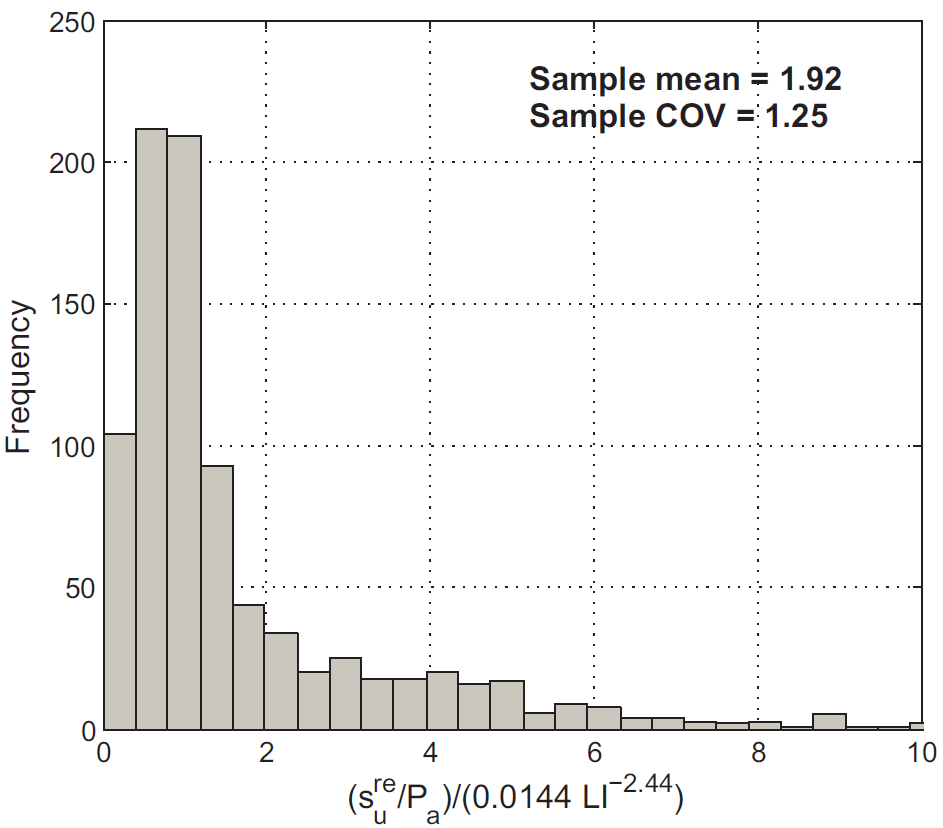
\includegraphics[width=0.5\textwidth]{figures/figure-15.png}
    \caption{Histogram of $(s_u^{re}/P_a)/(0.0144\rm{LI}^{-2.44})$.}
    \addtocounter{figure}{-1}
    \vspace{-5pt}
    \renewcommand{\figurename}{图}
    \caption{$(s_u^{re}/P_a)/(0.0144\rm{LI}^{-2.44})$的直方图。}
    \renewcommand{\figurename}{Figure}
    \label{figure:15}
\end{figure}
    \ParallelLText
    {
        where b is the bias factor ($b$ = 1 means unbiased) and $\epsilon$ is the variability term with mean = 1 and COV = $\delta$. If $\delta = 0$, there is no data scatter about the transformation model, i.e., the prediction is single-valued or deterministic, rather than a distribution. The $\rm{LI}-(s_u^{re}/P_a)$ model proposed by \citet{Locat1988799} is biased because the bias factor ($b$) is around 1.92, and the COV of this model is around 1.25. This model basically underpredicts the actual value by a factor of about 2 (conservative model). The uncertainty underlying this prediction when it is made to cover the wide range of conditions in the global database is considerable given that the COV exceeds 100$\%$. The calibrated bias factors and COVs for all models are shown in the last two columns of Table \ref{table:5}. The number of data points “$n$” used for each calibration is listed in the table.
    }
    \ParallelRText
    {
        式中$b$是偏差因子($b = 1$表示无偏),$\epsilon$是均值= 1且COV = $ \delta $的可变项。 如果$ \delta = 0 $,则没有关于转换模型的数据分散,即预测是单值或确定性的,而不是某种分布。 \citet{Locat1988799}提出的$\rm{LI}-(s_u^{re}/P_a)$模型是有偏差的,因为偏差因子($b$)约为1.92,而该模型的COV约为1.25。 该模型基本上将实际值低估了约2倍(保守模型)。 考虑到COV超过100%,当预测覆盖全球数据库中的广泛条件时,这种不确定性是相当大的。 表\ref{table:5}的最后两列显示了所有模型的校准偏差因子和COV。表中列出了每次校准使用的数据点“$n$”的数量。
    }
    \ParallelPar
    \ParallelLText
    {
        It is evident that models published in more recent studies, such as citet{Kulhawy1990}, \citet{Chen1996488}, and \citet{Ching201252, Ching2012522} mostly have bias factors $b\approx{}1$ (less biased). These recent studies compiled fairly large databases as well. It is also evident that the COVs ($\delta$) calibrated by the global database in this study are typically higher than those reported in the literature (see the numbers in the parentheses in the rightmost column in Table \ref{table:5}). The exceptions are the $\rm{LI}–S_t$, $\rm{LI}-(\sigma_p'/P_a)-S_t$ and $\rm{OCR}-(s_u/\sigma_v')-S_t$ models developed in \citet{Ching2012522}: COVs for these three models are close to those reported in \citet{Ching2012522}. The statistics of the database used by \citet{Ching2012522} are given in the “Remarks” column in Table \ref{table:5}. 
    }
    \ParallelRText
    {
        显然,在最近的研究中发表的模型,例如\citet{Kulhawy1990},\citet{Chen1996488}以及\citet{Ching201252, Ching2012522},大多具有偏差因子$b\approx{}1$(偏差较小)。 这些最近的研究也汇编了相当大的数据库。 同样明显的是,这项研究中由全球数据库校准的COV($\delta$)通常高于文献报道的COV(请参见表\ref{table:5}最右栏中的括号中的数字)。 \citet{Ching2012522}开发的$\rm{LI}–S_t$,$\rm{LI}-(\sigma_p'/P_a)-S_t$和$\rm{OCR}-(s_u/\sigma_v')-S_t$模型除外:这三个模型的COV接近\citet{Ching2012522}中报道的那些。\citet{Ching2012522}使用的数据库的统计信息在表\ref{table:5}的“备注”列中给出。
    }
    \ParallelPar
    \ParallelLText
    {
        The bias factors in Table \ref{table:5} still deviate somewhat from unity for two possible reasons:

        1. The bias factors in Table \ref{table:5} are calibrated using the global database in this study that contains broader types of clays, typically broader than the databases used to develop the transformation models in the literature. For instance, \citet{Ching2012522} only considered structured clays.

        2. All $s_u$ data points in the global database are converted to $s_u(\rm{mob})$ (see Table \ref{table:2}). Such a conversion step may introduce an extra bias.
    }
    \ParallelRText
    {
        表\ref{table:5}中的偏差因子仍因某些可能的原因而偏离统一性:

        1. 使用本研究中的全球数据库对表\ref{table:5}中的偏差因子进行校准,该数据库包含更广泛的黏土类型,通常比文献中用于开发转化模型的数据库更广泛。 例如,\citet{Ching2012522}仅考虑结构化黏土。
        
        2. 全局数据库中的所有$s_u$数据点都将转换为$s_u(\rm{mob})$(请参见表\ref{table:2})。 这样的转换步骤可能会引入额外的偏差。
    }
    \ParallelPar
    \ParallelLText
    {
        The COVs in Table \ref{table:5} are typically larger than those reported in the literature for three possible reasons:

        1. These COVs are calibrated using the global database that contains broader types of clays.

        2. The conversion of the $s_u$ data points to a reference strength, $s_u(\rm{mob})$, would introduce transformation uncertainty. It is noteworthy that the COVs can be even larger without this conversion, because su varies significantly with the test type \citep{Ladd1977421}.
        
        3. The COVs summarized in \citet{Ching201252} for the $\rm{CPTU}-(s_u/\sigma_v')$ transformation models do not include measurement errors.
    }
    \ParallelRText
    {
        由于以下三种可能的原因,表\ref{table:5}中的COV通常大于文献报道的COV:

        1. 使用包含更广泛类型的黏土的全球数据库对这些COV进行校准。

        2. 将$s_u$数据点转换为参考强度$s_u(\rm{mob})$,将引入转换不确定性。 值得注意的是,如果不进行这种转换,COV可能会更大,因为su随测试类型而变化很大\citep{Ladd1977421}。
       
        3. \citet{Ching201252}中针对$\rm{CPTU}-(s_u/\sigma_v')$转换模型总结的COV不包括测量误差。
    }
    \ParallelPar
    \ParallelLText
    {
        By definition, the models calibrated by the global database are unbiased with respect to the global database in this study. For instance, for the $\rm{LI}-s_u^{re}/P_a$ model by \cite{Locat1988799}, the predicted value for $s_u^{re}/P_a$ is $0.0144\rm{LI}^{-2.44}$. This model has a bias factor $b = 1.92$, calibrated by the global database. As a result, the calibrated model $s_u^{re}/P_a\approx{}b(0.0144)\rm{LI}^{-2.44}=1.92(0.0144)\rm{LI}^{-2.44}$ is an “unbiased prediction” with respect to the global database. This means that this calibrated model can capture the mean trend of the global database, and the calibrated COV can adequately capture the data scatter around the mean trend. However, the COV is typically quite large to capture the data scatter. In the next section, the possibility of incorporating secondary input parameters to reduce the COV is addressed.
    }
    \ParallelRText
    {
        根据定义,在本研究中,由全局数据库校准的模型相对于全局数据库没有偏见。 例如,对于\cite{Locat1988799}的$\rm{LI}-s_u^{re}/P_a$模型,$s_u^{re}/P_a$的预测值为$0.0144\rm{LI}^{-2.44}$。 该模型的偏差因子$b = 1.92$,已通过全局数据库进行了校准。 结果,校准后的模型$s_u^{re}/P_a\approx{}b(0.0144)\rm{LI}^{-2.44}=1.92(0.0144)\rm{LI}^{-2.44}$对于全局数据库而言是“无偏预测”。 这意味着该校准模型可以捕获全局数据库的平均趋势,并且校准COV可以充分捕获平均趋势周围的数据散布。 但是,COV通常很大以捕获数据散布。 在下一节中,讨论了合并次级输入参数以降低COV的可能性。
    }
\end{Parallel}